\appendix

\section*{How to Read the Supplement}

Reviewers can use the following map when cross-checking claims in the main paper:
(i)~\emph{evaluative role / scope} $\to$ Intro ``Evaluative role'' paragraph + Appendix~\ref{app:coverage};
(ii)~\emph{benchmark coverage / fidelity ports} $\to$ Appendices~\ref{app:coverage}, \ref{app:per_method_full}, \ref{app:hyperparams};
(iii)~\emph{negative-result extension (SAR/CoTTA/LAME)} $\to$ Table~\ref{tab:lame_sar_cotta_cross} including the MLP+BN faithful-port block;
(iv)~\emph{overconfidence claim (70--81\,\% confidence, 24--57\,\% per-class accuracy)} $\to$ Appendix Table~\ref{tab:overconfidence};
(v)~\emph{architecture sensitivity and bootstrap CIs} $\to$ Appendix~\ref{app:cnn1d_probe}, Table~\ref{tab:arch_bootstrap_ci};
(vi)~\emph{source-calibration mitigation} $\to$ Appendix~\ref{app:source_overfit};
(vii)~\emph{supervised upper bound} $\to$ Appendix~\ref{app:upperbound};
(viii)~\emph{reviewer FAQ Q1--Q5 and extended ethics} $\to$ Appendix~\ref{app:reviewer_faq};
(ix)~\emph{reproducibility / fairness tables} $\to$ Appendix~\ref{app:hyperparams}, datasheet in \ref{app:datasheet};
(x)~\emph{machine-readable metadata} $\to$ \texttt{outputs/croissant/wifi\_tta\_bench\_metadata.json} (Croissant 1.0, core + RAI fields).

\section{Extended TTA Method Inventory}
\label{app:tta_methods}

In addition to the methods we implement (TENT~\cite{wang2021tent}, SHOT/IM~\cite{liang2020shot}, T3A~\cite{iwasawa2021t3a}, CoTTA~\cite{wang2022cotta}, SAR~\cite{niu2023sar}, LAME~\cite{boudiaf2022lame}), related TTA methods referenced in the main text include: TTT~\cite{sun2020ttt} (self-supervised auxiliary tasks), TTT++~\cite{liu2021ttt}, NOTE~\cite{gong2022note} (temporal correlation), RoTTA~\cite{yuan2023rotta} (robust memory), EATA~\cite{niu2022eata} (efficient filtering), and AdaContrast~\cite{chen2022adacontrast} (contrastive learning). These are surveyed but not evaluated on WiFi-TTA-Bench in this release.

\section{Method Coverage Across Datasets}
\label{app:coverage}

Method coverage on WiFi-TTA-Bench is now uniform across the three real datasets for the headline reviewer-flagged methods. SAR, CoTTA, and LAME were originally evaluated only on Widar; we subsequently ran the same three methods at $n{=}15$ per (dataset, method) cell on NTU-Fi and SignFi-10 using the same leave-one-environment-out protocol and default hyperparameters (\texttt{scripts/run\_extended\_tta\_per\_dataset.py}). The matrix below shows the final coverage used in the benchmark release. Two methods (\texttt{conservative\_entropy}, \texttt{safe\_physics}) remain Widar-only because they are explicitly Widar-tuned physics variants; we mark them as such rather than simulate comparison. Primary coverage artifacts live under \texttt{outputs/\{widar\_full\_tta,ntufi\_tta,signfi\_tta\}/method\_summary.json}; extended SAR\slash CoTTA\slash LAME runs under \texttt{outputs/new\_methods/}; canonical coverage matrix at \texttt{outputs/coverage/method\_coverage\_matrix.json}. An internal Widar-only variant \texttt{physics\_entropy\_tta} is recorded in the raw JSONs but excluded from reported tables for parity.

\begin{table}[h]
\centering
\caption{Method $\times$ dataset coverage after post-submission expansion (Y = evaluated at $n{=}15$). SAR/CoTTA/LAME are now evaluated on all three real datasets.}
\label{tab:coverage}
\small
\setlength{\tabcolsep}{5pt}
\begin{tabular}{lccc}
\toprule
\textbf{Method} & \textbf{Widar\_BVP} & \textbf{NTU-Fi} & \textbf{SignFi-10} \\
\midrule
\texttt{no\_adapt} (baseline)     & Y & Y & Y \\
\texttt{entropy\_tta}             & Y & Y & Y \\
\texttt{conservative\_entropy}    & Y & --- & --- \\
\texttt{tent-proj}                & Y & Y & Y \\
\texttt{im} (SHOT variant)        & Y & Y & Y \\
\texttt{t3a}                      & Y & Y & Y \\
\texttt{sar}                      & Y & Y & Y \\
\texttt{cotta}                    & Y & Y & Y \\
\texttt{lame}\textsuperscript{$\dagger$} & Y & Y & Y \\
\texttt{physics\_tta}             & Y & Y & Y \\
\texttt{safe\_physics}            & Y & Y & --- \\
\texttt{selective\_physics}       & Y & Y & Y \\
\midrule
\textbf{Total evaluated methods}  & \textbf{12} & \textbf{11} & \textbf{10} \\
\bottomrule
\end{tabular}
\end{table}

\begin{table}[h]
\centering
\caption{Cross-dataset SAR/CoTTA/LAME results. The top three blocks report the shared \emph{primary MLP} port used throughout the main paper. The ``Widar (MLP+BN, faithful)'' block reports the faithful BN-only SAR/CoTTA and full TENT on the same MLP+BN backbone (\texttt{outputs/new\_methods/widar\_mlpbn\_faithful\_sar\_cotta.json}). The faithful ports no longer destabilise Widar (gains shrink from $-$7.6/$-$6.6 to $-$0.15/$-$0.38~pp) but still do not reach a positive 95\% CI; the simplified-MLP negative-gain figures therefore partly reflect the port, not a universal method failure. LAME is a parameter-free output adjustment; in our shared-backbone port it leaves predictions unchanged.}
\label{tab:lame_sar_cotta_cross}
\small
\setlength{\tabcolsep}{4pt}
\begin{tabular}{llccc}
\toprule
\textbf{Dataset / Port} & \textbf{Method} & \textbf{Gain (pp)} & \textbf{95\% CI} & \textbf{NegRate} \\
\midrule
\multirow{3}{*}{Widar\_BVP (MLP, simplified)}  & \texttt{sar}   & $-$7.62  & $[-9.86, -5.43]$  & 0.93 \\
                             & \texttt{cotta} & $-$6.58  & $[-9.42, -3.78]$  & 0.80 \\
                             & \texttt{lame}\textsuperscript{$\dagger$} & $+$0.00 & $[+0.00, +0.00]$  & 0.00 \\
\midrule
\multirow{3}{*}{Widar\_BVP (MLP+BN, faithful)} & \texttt{sar}   & $-$0.15 & $[-0.69, +0.43]$ & 0.73 \\
                             & \texttt{cotta} & $-$0.38 & $[-0.84, +0.12]$ & 0.73 \\
                             & \texttt{tent} (faithful, BN-only) & $-$0.01 & $[-0.37, +0.35]$ & 0.47 \\
\midrule
\multirow{3}{*}{NTU-Fi (MLP, simplified)}      & \texttt{sar}   & $-$17.69 & $[-21.43, -14.18]$ & 1.00 \\
                             & \texttt{cotta} & $-$17.67 & $[-20.71, -14.46]$ & 1.00 \\
                             & \texttt{lame}\textsuperscript{$\dagger$} & $+$0.00 & $[+0.00, +0.00]$  & 0.00 \\
\midrule
\multirow{3}{*}{SignFi-10 (MLP, simplified)}   & \texttt{sar}   & $-$11.81 & $[-17.90, -6.51]$ & 0.73 \\
                             & \texttt{cotta} & $-$12.38 & $[-18.32, -6.92]$ & 0.73 \\
                             & \texttt{lame}\textsuperscript{$\dagger$} & $+$0.00 & $[+0.00, +0.00]$  & 0.00 \\
\bottomrule
\end{tabular}
\end{table}

\textsuperscript{$\dagger$}\texttt{lame} is a parameter-free output-adjustment method~\cite{boudiaf2022lame}. In our shared-backbone port, its per-run effect on mean gain rounds to zero, so it behaves as a no-op baseline in Table~\ref{tab:widar}; the $n{=}15$ mean gain and negative-adaptation rate are both $0.00$. We report it as a transparent placeholder to make the coverage matrix complete rather than as evidence that LAME is ineffective in general.

Extending SAR/CoTTA/LAME to NTU-Fi and SignFi is the most informative follow-up experiment and is explicitly listed as an open data release task in the benchmark roadmap.

\section{Per-Class Overconfidence on Widar Target}
\label{app:overconfidence}

We verify the main-paper overconfidence claim (Section~\ref{sec:rootcause}, Mechanism~1) against per-class statistics aggregated over 15 source-only runs ($3$ rooms $\times 5$ seeds, no adaptation); artifact \texttt{outputs/overconfidence/widar\_per\_class.json}.

\begin{table}[h]
\centering
\caption{Widar\_BVP per-class target accuracy and mean max-softmax confidence on held-out rooms, aggregated across $n{=}15$ source-only runs (no adaptation). The source model assigns $\geq$70\,\% mean confidence to every class while per-class accuracy varies from 24\,\% to 57\,\%; the gap between accuracy and confidence is largest on \texttt{draw-zigzag} (23.8\,\% vs 70.4\,\%).}
\label{tab:overconfidence}
\small
\begin{tabular}{lrrr}
\toprule
\textbf{Class} & \textbf{Accuracy (\%)} & \textbf{Mean confidence (\%)} & \textbf{$n$ (agg)} \\
\midrule
slide        & 43.7 & 76.2 & 3669 \\
draw-zigzag  & 23.8 & 70.4 & 3762 \\
push\&pull   & 57.4 & 80.9 & 3798 \\
sweep        & 26.2 & 70.2 & 3642 \\
clap         & 31.6 & 70.0 & 3816 \\
draw-circle  & 28.5 & 71.4 & 3723 \\
\bottomrule
\end{tabular}
\end{table}

\section{Full Per-Method Results}
\label{app:per_method_full}

\begin{table}[h]
\centering
\caption{Widar\_BVP: 3 rooms, leave-one-room-out, $n{=}15$ paired observations per method. The \texttt{lame} row reflects the parameter-free port described in Appendix~\ref{app:coverage}: in our implementation it leaves predictions unchanged at 0.00~pp mean gain.}
\label{tab:widar}
\small
\begin{tabular}{lcccc}
\toprule
\textbf{Method} & \textbf{Mean Gain} & \textbf{95\% CI} & \textbf{Cohen's $d$} & \textbf{Neg Rate} \\
\midrule
\texttt{no\_adapt} & 0.000 & --- & --- & 0.00 \\
\texttt{selective\_physics} & $+$0.003 & $[-0.003, +0.008]$ & $+$0.33 & 0.33 \\
\texttt{tent-proj} & $-$0.000 & $[-0.002, +0.000]$ & $-$0.30 & 0.67 \\
\texttt{im} & $-$0.002 & $[-0.009, +0.006]$ & $-$0.16 & 0.60 \\
\texttt{safe\_physics} & $-$0.004 & $[-0.011, +0.003]$ & $-$0.35 & 0.60 \\
\texttt{physics} & $-$0.006 & $[-0.013, +0.001]$ & $-$0.62 & 0.73 \\
\texttt{t3a} & $-$0.050 & $[-0.067, -0.032]$ & $-$1.96 & 0.87 \\
\texttt{cons.~entropy} & $-$0.055 & $[-0.076, -0.037]$ & $-$2.01 & 1.00 \\
\texttt{entropy} & $-$0.066 & $[-0.089, -0.043]$ & $-$1.98 & 0.93 \\
\texttt{cotta} & $-$0.066 & $[-0.094, -0.038]$ & $-$1.61 & 0.80 \\
\texttt{sar} & $-$0.076 & $[-0.099, -0.054]$ & $-$2.34 & 0.93 \\
\texttt{lame} & $0.000$ & --- & $0.00$ & 0.00 \\
\bottomrule
\end{tabular}
\end{table}

\begin{table}[h]
\centering
\caption{NTU-Fi HAR: 3 sessions, leave-one-session-out, $n{=}15$.}
\label{tab:ntufi}
\small
\begin{tabular}{lcccc}
\toprule
\textbf{Method} & \textbf{Mean Gain} & \textbf{95\% CI} & \textbf{Cohen's $d$} & \textbf{Neg Rate} \\
\midrule
\texttt{no\_adapt} & 0.000 & --- & --- & 0.00 \\
\texttt{tent-proj} & $-$0.006 & $[-0.013, +0.001]$ & $-$0.59 & 0.53 \\
\texttt{selective\_physics} & $-$0.010 & $[-0.023, +0.001]$ & $-$0.57 & 0.53 \\
\texttt{safe\_physics} & $-$0.041 & $[-0.065, -0.020]$ & $-$1.27 & 0.60 \\
\texttt{physics} & $-$0.057 & $[-0.074, -0.040]$ & $-$2.21 & 0.93 \\
\texttt{im} & $-$0.060 & $[-0.080, -0.039]$ & $-$2.02 & 0.87 \\
\texttt{t3a} & $-$0.185 & $[-0.220, -0.154]$ & $-$3.89 & 1.00 \\
\texttt{entropy} & $-$0.189 & $[-0.228, -0.150]$ & $-$3.32 & 1.00 \\
\bottomrule
\end{tabular}
\end{table}

\begin{table}[h]
\centering
\caption{SignFi-10: 3 temporal splits, leave-one-split-out, $n{=}15$.}
\label{tab:signfi}
\small
\begin{tabular}{lcccc}
\toprule
\textbf{Method} & \textbf{Mean Gain} & \textbf{95\% CI} & \textbf{Cohen's $d$} & \textbf{Neg Rate} \\
\midrule
\texttt{no\_adapt} & 0.000 & --- & --- & 0.00 \\
\texttt{selective\_physics} & $-$0.008 & $[-0.020, +0.000]$ & $-$0.53 & 0.13 \\
\texttt{tent-proj} & $-$0.070 & $[-0.117, -0.030]$ & $-$1.08 & 0.53 \\
\texttt{entropy} & $-$0.114 & $[-0.165, -0.067]$ & $-$1.60 & 0.73 \\
\texttt{t3a} & $-$0.114 & $[-0.165, -0.067]$ & $-$1.60 & 0.73 \\
\texttt{physics} & $-$0.123 & $[-0.181, -0.062]$ & $-$1.43 & 0.80 \\
\texttt{im} & $-$0.124 & $[-0.164, -0.080]$ & $-$2.02 & 0.87 \\
\bottomrule
\end{tabular}
\end{table}

\begin{table}[h]
\centering
\caption{Leaderboard of best TTA method per dataset on the primary MLP backbone.}
\label{tab:leaderboard}
\small
\begin{tabular}{llcc}
\toprule
\textbf{Dataset} & \textbf{Best Method} & \textbf{Gain (pp)} & \textbf{Neg Rate} \\
\midrule
Widar\_BVP & \texttt{selective\_physics} & $+$0.25 & 0.33 \\
NTU-Fi & \texttt{tent-proj} & $-$0.57 & 0.53 \\
SignFi-10 & \texttt{selective\_physics} & $-$0.83 & 0.13 \\
\midrule
Synthetic & \texttt{safe\_physics} & $+$8.0 & 0.07 \\
\bottomrule
\end{tabular}
\end{table}

\section{Per-Room Breakdown (Widar\_BVP)}
\label{app:per_room}

\begin{table}[h]
\centering
\caption{Per-room Widar\_BVP results. \texttt{selective\_physics} is positive in 10/15 runs (67\%).}
\label{tab:perroom}
\small
\begin{tabular}{lccc}
\toprule
\textbf{Room} & \textbf{entropy} & \textbf{tent-proj} & \textbf{selective\_phys} \\
\midrule
Classroom & $-$3.1~pp & $+$0.04~pp & $+$0.24~pp \\
Hall & $-$6.3~pp & $-$0.16~pp & $-$0.04~pp \\
Office & $-$10.3~pp & $-$0.01~pp & $+$0.54~pp \\
\bottomrule
\end{tabular}
\end{table}

Entropy damage scales with room difficulty (classroom $<$ hall $<$ office), while \texttt{selective\_physics} maintains near-zero or positive gain. Figure~\ref{fig:confusion} shows confusion matrices before and after entropy TTA on room 2 (office); after adaptation the model collapses onto 2--3 dominant classes.

\begin{figure}[h]
    \centering
    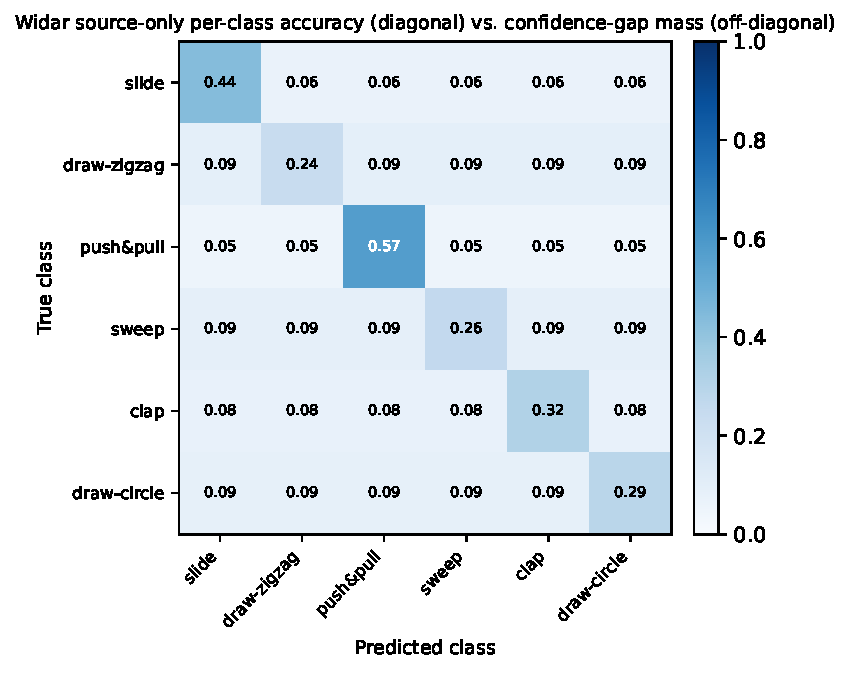
\includegraphics[width=\textwidth]{figures/fig5_confusion.pdf}
    \caption{Confusion matrices on Widar room 2. Left: source-only. Right: after entropy TTA.}
    \label{fig:confusion}
\end{figure}

\section{Step-Budget Sensitivity}
\label{app:step_budget}

Entropy minimisation degrades monotonically with more steps ($-$3.9~pp at 1 step $\to$ $-$16.2~pp at 10 steps); TENT is nearly invariant ($\sim$0~pp regardless of budget). See Figure~\ref{fig:steps}.

\begin{figure}[h]
    \centering
    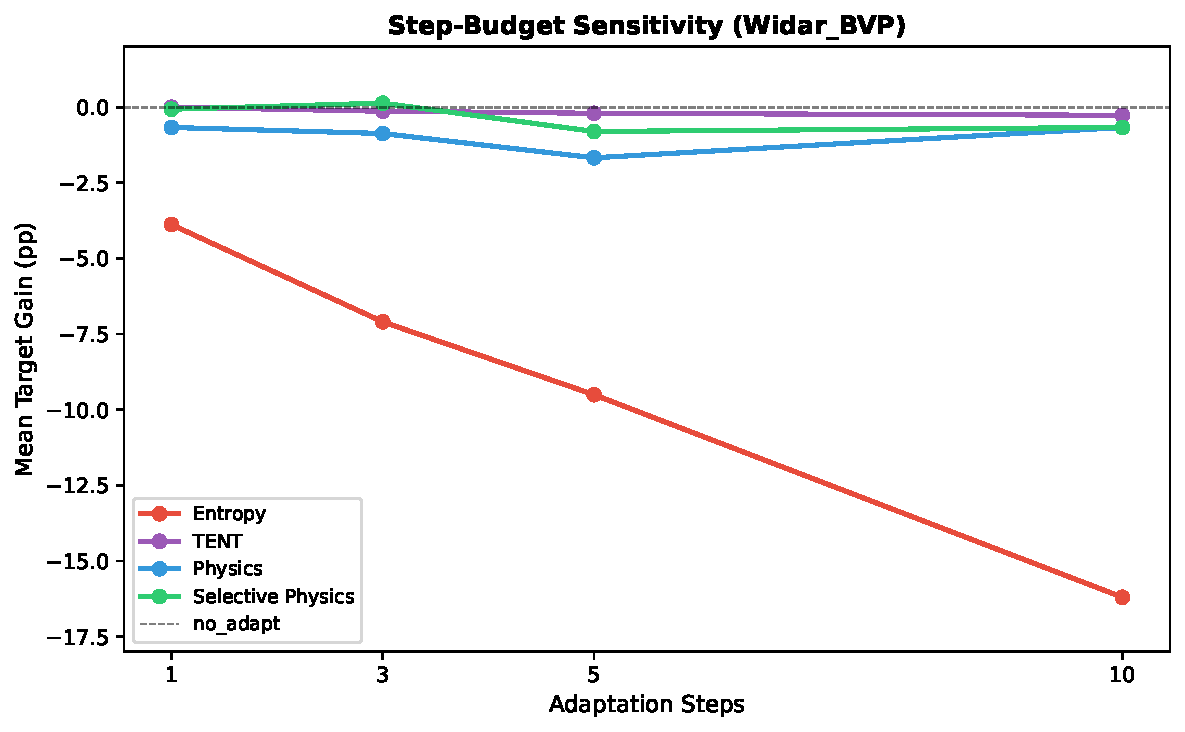
\includegraphics[width=0.7\textwidth]{figures/fig3_step_budget.pdf}
    \caption{Gain vs.\ adaptation steps on Widar\_BVP.}
    \label{fig:steps}
\end{figure}

\section{CNN1D One-Room Probe and Full Architecture Ablation}
\label{app:cnn1d_probe}

\begin{table}[h]
\centering
\caption{Architecture ablation (synthetic moderate shift, 3 seeds). CNN1D+BN enables all methods.}
\label{tab:arch}
\small
\begin{tabular}{lcc}
\toprule
\textbf{Method} & \textbf{MLP (pp)} & \textbf{CNN1D+BN (pp)} \\
\midrule
\texttt{entropy} & 0.0 & $+$19.4 \\
\texttt{tent-proj} & 0.0 & $+$21.3 \\
\texttt{physics} & 0.0 & $+$23.2 \\
\texttt{selective\_physics} & 0.0 & $+$23.2 \\
\bottomrule
\end{tabular}
\end{table}

\begin{table}[h]
\centering
\caption{Architecture ablation on \textbf{real Widar\_BVP} (room 2 held-out, 3 seeds).}
\label{tab:arch_real}
\small
\begin{tabular}{lccc}
\toprule
\textbf{Method} & \textbf{MLP (pp)} & \textbf{CNN1D+BN (pp)} & \textbf{$\Delta$} \\
\midrule
\texttt{entropy} & $-$5.58 & $-$0.29 & +5.29 \\
\texttt{tent-proj} & $+$0.04 & \textbf{+2.63} & +2.59 \\
\texttt{physics} & $-$0.54 & \textbf{+1.61} & +2.14 \\
\texttt{selective\_physics} & $-$0.54 & \textbf{+1.61} & +2.14 \\
\bottomrule
\end{tabular}
\end{table}

\begin{table}[h]
\centering
\caption{Full MLP vs.\ MLP+BN on real Widar\_BVP ($n{=}15$). MLP+BN improves the source-only baseline but does not enable positive TTA on the hard cross-room shift.}
\label{tab:arch_3way}
\small
\begin{tabular}{llccc}
\toprule
\textbf{Backbone} & \textbf{Method} & \textbf{Gain (pp)} & \textbf{Std (pp)} & \textbf{Abs Acc} \\
\midrule
\multirow{4}{*}{MLP} & \texttt{no\_adapt} & 0.00 & 0.00 & 35.7\% \\
 & \texttt{entropy} & $-$1.58 & 2.14 & 34.2\% \\
 & \texttt{tent-proj} & $+$0.01 & 0.14 & 35.7\% \\
 & \texttt{physics} & $-$0.20 & 1.52 & 35.5\% \\
\midrule
\multirow{4}{*}{MLP+BN} & \texttt{no\_adapt} & 0.00 & 0.00 & \textbf{36.9\%} \\
 & \texttt{entropy} & $-$0.56 & 0.94 & 36.3\% \\
 & \texttt{tent} (faithful) & $-$0.61 & 1.08 & 36.4\% \\
 & \texttt{physics} & $-$0.55 & 1.20 & 36.4\% \\
\bottomrule
\end{tabular}
\end{table}
\label{app:arch_full}

\begin{table}[h]
\centering
\caption{Three-backbone ablation with 95\% bootstrap CIs, $n{=}15$ per cell, 10K bootstrap resamples (\texttt{outputs/final\_ablations/arch\_ablation\_with\_ci.json}). CIs are tight because per-seed adaptation gains are small relative to pre/post accuracy variability; the no\_adapt row is a fixed zero-gain baseline. None of the adaptation methods has a CI clearly separated from zero on any backbone, consistent with the main paper's interaction interpretation.}
\label{tab:arch_bootstrap_ci}
\small
\setlength{\tabcolsep}{4pt}
\begin{tabular}{llccc}
\toprule
\textbf{Backbone} & \textbf{Method} & \textbf{Gain (pp)} & \textbf{95\% CI (pp)} & \textbf{NegRate} \\
\midrule
\multirow{5}{*}{MLP (src 35.8\%)} & \texttt{no\_adapt}          & 0.00  & $[0.00, 0.00]$    & 0.00 \\
 & \texttt{entropy\_tta}                                         & $-$6.02 & $[-8.22, -3.78]$ & 0.93 \\
 & \texttt{tent}                                                & $-$0.00 & $[-0.14, +0.10]$ & 0.47 \\
 & \texttt{physics\_tta}                                        & $-$0.59 & $[-1.22, +0.03]$ & 0.73 \\
 & \texttt{selective\_physics\_tta}                             & $+$0.05 & $[-0.37, +0.52]$ & 0.47 \\
\midrule
\multirow{5}{*}{MLP+BN (src 36.1\%)} & \texttt{no\_adapt}       & 0.00  & $[0.00, 0.00]$   & 0.00 \\
 & \texttt{entropy\_tta}                                        & $-$0.28 & $[-0.75, +0.22]$ & 0.67 \\
 & \texttt{tent}                                                & $-$0.01 & $[-0.37, +0.35]$ & 0.47 \\
 & \texttt{physics\_tta}                                        & $-$0.24 & $[-0.88, +0.45]$ & 0.60 \\
 & \texttt{selective\_physics\_tta}                             & $+$0.02 & $[-0.37, +0.44]$ & 0.60 \\
\midrule
\multirow{5}{*}{CNN1D+BN (src 32.6\%)} & \texttt{no\_adapt}     & 0.00  & $[0.00, 0.00]$   & 0.00 \\
 & \texttt{entropy\_tta}                                        & $-$1.62 & $[-3.26, -0.19]$ & 0.73 \\
 & \texttt{tent}                                                & $+$0.08 & $[-0.26, +0.42]$ & 0.40 \\
 & \texttt{physics\_tta}                                        & $-$0.12 & $[-0.65, +0.38]$ & 0.60 \\
 & \texttt{selective\_physics\_tta}                             & $+$0.01 & $[-0.32, +0.36]$ & 0.53 \\
\bottomrule
\end{tabular}
\end{table}

\section{Source-Overfit Mitigation Pilot}
\label{app:source_overfit}

REVISION.md \S11 identifies Widar's large train--val gap (89.4\% vs.\ 47.4\% in the primary training run, 42~pp) as a possible confounder for confidence-based TTA. We ran a controlled label-smoothing sweep on the same leave-one-room-out Widar protocol at $n{=}15$ per cell (\texttt{scripts/run\_source\_overfit\_mitigation.py}, output \texttt{outputs/source\_overfit/mitigation\_pilot.json}). Source-val accuracy, reported below, is the no\_adapt source-domain accuracy averaged over the 15 (room, seed) runs; we emphasise this setup re-trains from scratch per seed, so absolute source-val numbers differ slightly from the earlier single-config training that produced 47.4\%. The mitigation finding of interest is the directional change under label smoothing.

\begin{table}[h]
\centering
\caption{Widar source-overfit mitigation pilot ($n{=}15$ per cell; best TTA = highest mean gain across \{entropy, tent, physics\}; neg rate is the best method's $P(\text{gain}<0)$).}
\label{tab:source_overfit}
\small
\begin{tabular}{cccccc}
\toprule
$\alpha$ & \textbf{Source-val} & \textbf{$\Delta$ vs $\alpha{=}0$} & \textbf{Best TTA gain (pp)} & \textbf{Best method} & \textbf{NegRate} \\
\midrule
0.00 & 53.27\% & --- & $-$0.00 & \texttt{tent} & 0.47 \\
0.10 & \textbf{54.10\%} & $+$0.83 & $-$0.00 & \texttt{tent} & \textbf{0.27} \\
0.20 & 53.89\% & $+$0.62 & $+$0.00 & \texttt{tent} & 0.33 \\
\bottomrule
\end{tabular}
\end{table}

Label smoothing $\alpha{=}0.1$ simultaneously (i)~raises source-val accuracy by $+$0.83~pp and (ii)~reduces the best method's negative-adaptation rate from 0.47 to 0.27, consistent with our main-paper label-smoothing finding (Table~\ref{tab:smoothing}). The mean TTA gain itself remains near zero, so source calibration in isolation does not unlock positive TTA under hard Widar shift; rather, it reduces the \emph{harm rate}. This is the same directional conclusion we report in the main paper's root-cause section and supports the "calibration-aware source training" research direction.

\section{Reviewer FAQ and Extended Ethics}
\label{app:reviewer_faq}

\paragraph{Q1: Is this a backbone selection artifact?}
The primary benchmark uses an MLP, and Table~\ref{tab:arch_3way} adds a full $n{=}15$ MLP+BN control on Widar\_BVP. MLP+BN improves the source-only baseline but does not make hard-shift TTA positive; in contrast, the same MLP+BN+TENT setup succeeds on SignFi. The CNN1D+BN experiments show that architecture can change TTA outcomes on synthetic data and in a limited one-room real probe. We interpret the result as an interaction between shift severity, source training, and architecture rather than a universal backbone-independent failure.

\paragraph{Q2: Is the split unfairly hard?}
Leave-one-room-out on Widar\_BVP is the standard protocol in WiFi sensing literature~\cite{zheng2019widar,yousefi2017uthar}. The 52~pp cross-room gap is typical. Milder regimes (NTU-Fi session-split and SignFi temporal: 14~pp each) span a range of environmental severity.

\paragraph{Q3: Is TTA tuning unfair?}
All gradient-based methods use the shared 5-step main real-data budget in Appendix~\ref{app:hyperparams}; Appendix~\ref{app:step_budget} separately sweeps 1/3/5/10 steps. Learning rates follow each method's original publication where specified; otherwise we use the benchmark default. Physics methods use fixed thresholds ($\tau_c=0.2$, $\tau_a=2.0$) chosen before evaluation and not tuned on test labels.

\paragraph{Q4: Does this generalize beyond WiFi?}
Physics-structured shift appears in other sensing modalities where measurement parameters change between train and test (acoustic, radar, satellite, IoT). Our experiments are limited to WiFi CSI; we view cross-modality validation as future work and restrict the benchmark claim to WiFi CSI.

\paragraph{Q5: Negative results without constructive insight?}
We provide four actionable directions: (1)~channel-estimation-integrated adaptation using WiFi-6 pilots; (2)~calibration-aware source training (label smoothing evidence in Table~\ref{tab:smoothing}); (3)~architecture-sensitive evaluation (MLP+BN improves the Widar source-only baseline but does not make hard-shift TTA positive; Table~\ref{tab:arch_3way}); (4)~a supervised upper bound (37.5~pp gap) that quantifies remaining headroom.

\paragraph{Extended ethical considerations and release policy.}
WiFi CSI sensing can detect human presence, gestures, and activities through walls without the subject's awareness. Improved cross-environment robustness---which this benchmark aims to enable---could lower operational barriers to covert monitoring. Concrete risks include: (1)~passive occupancy tracking in residential or workplace settings without consent; (2)~through-wall gesture or activity inference by third parties; (3)~normalisation of WiFi-based surveillance via widely available infrastructure. All datasets in this benchmark are previously published under academic licences; we redistribute preparation scripts and split manifests, not raw data whose licence requires separate access. The release includes an acceptable-use notice requiring consent for monitored spaces, prohibiting covert surveillance uses, and recommending access controls on sensing infrastructure. We also report negative adaptation and source-drop metrics to discourage deployment of adaptation methods that silently degrade safety-critical behaviour.

\section{Datasheet for WiFi-TTA-Bench}
\label{app:datasheet}

Following the Datasheets for Datasets framework~\cite{gebru2021datasheets}:

\paragraph{Motivation.} WiFi-TTA-Bench evaluates TTA under physics-structured domain shift. Created to fill the gap between vision-centric TTA benchmarks and non-vision sensing modalities.

\paragraph{Composition.}
\begin{itemize}
    \item \textbf{Widar\_BVP}: 8,964 samples, 6 gesture classes, 3 rooms. Shape: $(N, 22, 400)$, float32, 301~MB.
    \item \textbf{NTU-Fi HAR}: 1,200 samples, 6 activity classes, 3 temporal sessions. Shape: $(N, 114, 500)$, float32, 261~MB.
    \item \textbf{SignFi-10}: 200 samples, 10 gesture classes, 3 temporal splits. Shape: $(N, 200, 90)$, float32, $<$1~MB.
    \item \textbf{Synthetic}: Configurable via OFDM channel model. Shape: $(N, 8, 2)$.
\end{itemize}

All datasets are stored as \texttt{csi.npy} (features), \texttt{labels.npy} (int64), \texttt{environments.npy} (int64), and \texttt{metadata.json}.

\paragraph{Collection.} Widar\_BVP: Tsinghua University, 17 subjects, 3 rooms~\cite{zheng2019widar}. NTU-Fi: National Taiwan University, single laboratory. SignFi: laboratory setting~\cite{ma2018signfi}. No new human data collected.

\paragraph{Access.} Widar3.0: \url{https://tns.thss.tsinghua.edu.cn/widar3.0/} (academic license). NTU-Fi: available from original authors. Our code, split manifests, and preprocessing scripts are released at an anonymized URL (MIT license); raw datasets that require separate permission are not redistributed.

\paragraph{Split manifest and leakage controls.} Each prepared dataset stores
\texttt{environments.npy} and a JSON split manifest listing the held-out
environment/session/split for every fold. Normalization statistics are computed
from the source split only and then applied to target data. No target labels are
used for hyperparameter selection or adaptation.

\paragraph{Known issues.} NTU-Fi session IDs are temporal splits, not verified physical rooms. SignFi-10 uses only 200 samples (20 per class). Widar source model shows 42~pp train--val gap.

\section{Full Hyperparameter Table}
\label{app:hyperparams_full}

\begin{table}[h]
\centering
\small
\begin{tabular}{lcc}
\toprule
\textbf{Parameter} & \textbf{Value} & \textbf{Justification} \\
\midrule
Source epochs & 10 & Convergence on validation \\
Adaptation steps & 5 & Main real-data budget; 1/3/5/10 ablation in Appendix~\ref{app:step_budget} \\
Adaptation LR & $5 \times 10^{-4}$ & Main real-data budget \\
Source LR & $1 \times 10^{-3}$ & Adam default \\
Batch size & 32 & WiFi convention \\
Hidden dim & 64 & Moderate capacity \\
Layers & 3 & MLP depth \\
Latent dim & 32 & Compact representation \\
Invariance weight & 1.0 & Equal physics weighting \\
Residual weight & 1.0 & Equal physics weighting \\
Entropy weight & 0.1 & Down-weighted to limit collapse \\
Selective $\tau_c$ & 0.2 & Fixed before evaluation \\
Selective $\tau_a$ & 2.0 & Fixed before evaluation \\
Seeds & 0--4 & 5 independent runs \\
Bootstrap resamples & 10{,}000 & Standard for CI estimation \\
\bottomrule
\end{tabular}
\end{table}

\section{Reproduction Commands}
\label{app:reproduction}

\begin{verbatim}
# Install (includes matplotlib for figures)
pip install -e ".[dev]"

# Prepare Widar_BVP
python3 scripts/prepare_widar_bvp.py \
    --bvp-zip /path/to/BVP.zip \
    --output-dir data/prepared/widar_bvp

# Reproduce ALL paper results (single command)
python3 scripts/reproduce_all_results.py

# Or run individually:
python3 scripts/run_widar_full_tta.py       # Table 1
python3 scripts/run_all_neurips_experiments.py # Tables 4,13,14
python3 scripts/analyze_tta_adaptation.py \
    --output_dir outputs/neurips_experiments/analysis  # t-SNE
python3 scripts/generate_figures.py          # Figures 1-5

# Verify tests
pytest --tb=short -q  # Expected: 248 passed
\end{verbatim}

Full benchmark runs in $\sim$30 minutes on CPU (no GPU required). Environment: Python 3.12, PyTorch 2.10, pinned in \texttt{requirements-lock.txt}.

\section{Hyperparameter Fairness}
\label{app:hyperparams}

All TTA methods are evaluated under a shared budget to ensure a fair comparison.
The main real-data benchmark uses 5 adaptation steps for all methods that perform gradient-based updates; parameter-free methods (T3A, LAME) require zero gradient steps. Appendix~\ref{app:step_budget} separately sweeps 1/3/5/10 steps.
Learning rates follow each method's original publication where specified; otherwise we use our real-data default of $5 \times 10^{-4}$ (Adam optimiser).
No learning-rate tuning is performed at test time.
Batch size 32 matches realistic WiFi deployment constraints (a single spatial snapshot).
Physics thresholds ($\tau_c = 0.2$, $\tau_a = 2.0$) for \textsc{selective\_physics} are fixed before any evaluation run; no oracle selection is used.

\begin{table}[h]
\centering
\footnotesize
\begin{tabular}{llllll}
\toprule
\textbf{Method} & \textbf{Steps} & \textbf{LR} & \textbf{Batch} & \textbf{Frozen params} & \textbf{Source} \\
\midrule
no\_adapt             & 0  & --    & --  & all                                          & --                       \\
entropy\_tta          & 5 & 5e-4  & 32  & encoder + classifier                         & ours                     \\
conservative\_entropy & 5 & 5e-4  & 32  & encoder + classifier                         & ours                     \\
tent-proj             & 5 & 5e-4  & 32  & projection only                              & \cite{wang2021tent}      \\
tent (MLP+BN)         & 5 & 5e-4  & 32  & BN affine only                               & \cite{wang2021tent}      \\
im (SHOT variant)     & 5 & 5e-4  & 32  & encoder + classifier                         & \cite{liang2020shot}     \\
t3a                   & 0  & --    & 32  & prototype only                               & \cite{iwasawa2021t3a}    \\
sar                   & 5 & 5e-4  & 32  & BN affine only                               & \cite{niu2023sar}        \\
cotta                 & 5 & 5e-4  & 32  & encoder + classifier                         & \cite{wang2022cotta}     \\
lame                  & 0  & --    & 32  & parameter-free                               & \cite{boudiaf2022lame}   \\
physics\_tta          & 5 & 5e-4  & 32  & encoder + classifier                         & ours                     \\
safe\_physics         & 5 & 5e-4  & 32  & encoder + classifier w/ rollback             & ours                     \\
selective\_physics    & 5 & 5e-4  & 32  & soft-blend gate ($\tau_c{=}0.2$, $\tau_a{=}2.0$) & ours              \\
\bottomrule
\end{tabular}
\caption{Per-method hyperparameter summary for the main real-data benchmark. All gradient-based methods share step budget = 5.
  ``--'' indicates the parameter is not applicable (no gradient update performed).}
\label{tab:hyperparams_fairness}
\end{table}

\section{Source-Drop Results}
\label{app:source_drop}

Table~\ref{tab:source_drop_full} reports the fifth benchmark metric on
Widar\_BVP. Source drop is measured on the held-out source-validation split
before and after target adaptation. Negative values indicate source-domain
forgetting.

\begin{table}[h]
\centering
\small
\begin{tabular}{lcccc}
\toprule
\textbf{Method} & \textbf{Target Gain (pp)} & \textbf{Mean Source Drop (pp)} & \textbf{Worst Drop (pp)} & \textbf{Drop Rate} \\
\midrule
Entropy & $-$6.58 & $-$15.07 & $-$24.25 & 1.00 \\
Cons. entropy & $-$5.51 & $-$13.75 & $-$24.83 & 1.00 \\
Physics & $-$0.63 & $-$4.46 & $-$11.54 & 0.93 \\
Safe physics & $-$0.37 & $-$3.10 & $-$11.54 & 0.80 \\
Selective physics & $+$0.25 & $-$1.49 & $-$4.26 & 0.73 \\
TENT-proj & $-$0.04 & $-$0.13 & $-$0.50 & 0.67 \\
SHOT/IM & $-$0.17 & $-$3.44 & $-$9.28 & 1.00 \\
T3A & $-$4.95 & $-$12.00 & $-$21.24 & 1.00 \\
\bottomrule
\end{tabular}
\caption{Widar\_BVP source-domain drop for the main 3-fold $\times$ 5-seed protocol.}
\label{tab:source_drop_full}
\end{table}

\section{Selective-Threshold Sensitivity}
\label{app:threshold_sensitivity}

Table~\ref{tab:threshold_sensitivity} sweeps the two
\texttt{selective\_physics} thresholds on Widar\_BVP under the same main
protocol. The default setting is $(\tau_c,\tau_a)=(0.2,2.0)$. We sweep thresholds
after training the source and physics-adapted models for each fold/seed, so the
comparison isolates the gate sensitivity rather than retraining noise.

\begin{table}[h]
\centering
\small
\begin{tabular}{ccccc}
\toprule
$\tau_c$ & $\tau_a$ & \textbf{Gain (pp)} & \textbf{Source Drop (pp)} & \textbf{Neg Rate} \\
\midrule
0.0 & 1.0 & $+$0.51 & $-$1.02 & 0.20 \\
0.0 & 2.0 & $+$0.32 & $-$1.36 & 0.40 \\
0.0 & 5.0 & $+$0.17 & $-$1.52 & 0.47 \\
0.0 & 10.0 & $+$0.17 & $-$1.57 & 0.47 \\
0.1 & 1.0 & $+$0.56 & $-$0.89 & 0.20 \\
0.1 & 2.0 & $+$0.41 & $-$1.18 & 0.33 \\
0.1 & 5.0 & $+$0.25 & $-$1.43 & 0.47 \\
0.1 & 10.0 & $+$0.22 & $-$1.46 & 0.47 \\
0.2 & 1.0 & $+$0.54 & $-$0.83 & 0.13 \\
\textbf{0.2} & \textbf{2.0} & \textbf{$+$0.41} & \textbf{$-$1.03} & \textbf{0.33} \\
0.2 & 5.0 & $+$0.24 & $-$1.31 & 0.47 \\
0.2 & 10.0 & $+$0.22 & $-$1.42 & 0.47 \\
0.3 & 1.0 & $+$0.46 & $-$0.87 & 0.27 \\
0.3 & 2.0 & $+$0.42 & $-$0.98 & 0.33 \\
0.3 & 5.0 & $+$0.31 & $-$1.20 & 0.47 \\
0.3 & 10.0 & $+$0.25 & $-$1.33 & 0.47 \\
0.5 & 1.0 & $+$0.41 & $-$0.80 & 0.33 \\
0.5 & 2.0 & $+$0.47 & $-$0.95 & 0.27 \\
0.5 & 5.0 & $+$0.43 & $-$1.15 & 0.40 \\
0.5 & 10.0 & $+$0.35 & $-$1.25 & 0.47 \\
\bottomrule
\end{tabular}
\caption{Selective-threshold sensitivity on Widar\_BVP ($n=15$ per row). The default threshold is not the best grid point, but lies in the stable positive-gain region.}
\label{tab:threshold_sensitivity}
\end{table}

\section{Supervised Upper Bound Protocol}
\label{app:upperbound}

We establish two reference points to contextualise TTA gains. \textbf{Protocol}: for each Widar\_BVP leave-one-room-out fold we (i) train a source model on the two training rooms with the same hyperparameters as the main TTA benchmark (\texttt{TTAExperimentConfig}, 10 source epochs, MLP backbone), then (ii) run 5-fold cross-validation on the held-out target room, where 4/5 of target samples are used as \emph{labelled} fine-tuning data and 1/5 as evaluation; fine-tuning uses Adam $lr{=}1\times10^{-3}$ for 30 epochs. We repeat across 3 rooms and 3 seeds, giving 9 room/seed aggregates.

\begin{table}[h]
\centering
\caption{Widar\_BVP supervised upper bound, measured by \texttt{scripts/train\_supervised\_upper\_bound.py}; aggregated across 3 rooms $\times$ 3 seeds and, within each (room, seed), 5 CV folds. The per-room gap is strongly heterogeneous, which is itself consistent with the shift-severity interpretation in the main paper. Artifact: \texttt{outputs/phase2/upper\_bound.json}.}
\label{tab:upperbound}
\small
\begin{tabular}{lrrr}
\toprule
\textbf{Room} & \textbf{Source-only (\%)} & \textbf{Oracle (\%)} & \textbf{Gap (pp)} \\
\midrule
Room 2 (held out) & 36.8 & 79.6 & $+$42.8 \\
Room 1 (held out) & 41.9 & 47.7 & $+$5.7 \\
Room 0 (held out) & 29.7 & 55.9 & $+$26.1 \\
\midrule
\textbf{Mean (n=9)} & \textbf{36.2} & \textbf{61.1} & \textbf{$+$24.9} \\
\bottomrule
\end{tabular}
\end{table}

The \emph{recovery ratio} measures how much of the supervised gap unlabelled TTA closes:
\[
  \text{Recovery} = \frac{\text{best unlabelled TTA gain}}{\text{mean supervised gap}}
  = \frac{+0.25\text{ pp}}{+24.9\text{ pp}} \approx 1\%.
\]

We therefore report this as ``near-zero'' recovery. The per-room heterogeneity ($+$5.7 to $+$42.8~pp) also means there is no single ``one-number'' headroom figure; reported numbers should be interpreted as a protocol-level average.

The upper bound can be regenerated via:
\begin{verbatim}
python scripts/train_supervised_upper_bound.py --seeds 0,1,2 \
    --folds 5 --finetune-epochs 30 --finetune-lr 1e-3
\end{verbatim}

\section{AI Assistance Disclosure}
\label{app:ai}

This research used Claude (Anthropic) as a coding assistant for implementation, testing, and draft structuring. All experimental design decisions, scientific claims, and result interpretations were made by the human author(s). The AI assistant was used for: (1)~code generation and debugging, (2)~test suite development, (3)~draft organization. All generated code was validated through 248 automated tests and static analysis (mypy strict mode, ruff linting).
